% 05-experiments.tex — 实验评估

\section{实验评估}
\label{sec:experiments}

\subsection{实验设置}

所有演化实验均在浏览器内通过 WebGPU compute shader 加速的 $(\mu+\lambda)$ 进化策略 (ES) 完成。两个 sweep 的参数对比如表~\ref{tab:es-params}。

\begin{table}[H]
\centering\small
\caption{两个 sweep 的 ES 演化参数对比}
\label{tab:es-params}
\begin{tabular}{lcc}
\toprule
\textbf{参数} & \textbf{小范围 sweep} & \textbf{大范围 sweep} \\
\midrule
种群规模 (pop)     & 200   & 500   \\
演化代数 (gens)    & 500   & 2000  \\
网格尺寸           & 40$\times$60 & 500$\times$2000 \\
mask 模板数        & 8     & 1 (manhattan-2) \\
maxFam 上限        & 1 / 2 / 4 / 8 & 8  \\
随机种子数         & 4     & 5 (s444, s1111, s2222, s3333, s5555) \\
总 run 数          & 128   & 5 \\
成功 run           & 122   & 5 \\
\bottomrule
\end{tabular}
\end{table}

小范围 sweep ($40 \times 60$) 完成 $8 \times 4 \times 4 = 128$ 次全交叉 run, 6 次因预算超时被剔除, 实际 122 OK; 大范围 sweep ($500 \times 2000$) 完成 5/5 run, 网格面积约高 170 倍, 用于验证 manhattan-2 / maxFam=8 在大网格上的 scale-up 能力。

\subsection{大范围 sweep 5 个随机种子结果}

\begin{figure}[H]
\centering
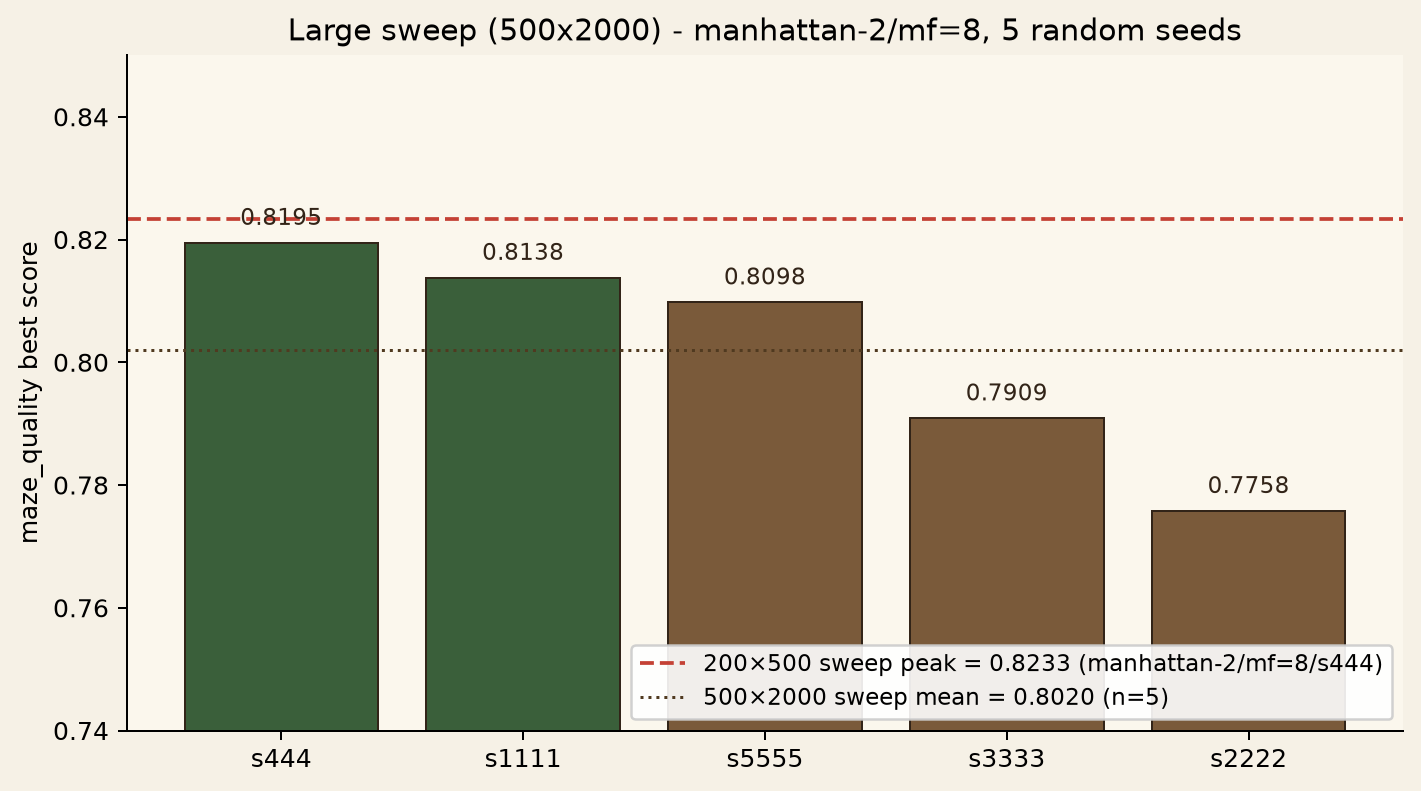
\includegraphics[width=0.96\linewidth]{../figures/v2/fig_bigsweep_top5.png}
\caption{\textbf{大范围 sweep ($500 \times 2000$) 5 个随机种子最优分。}
5 个 run 全部完成 (gen=2000 达代上限), 均使用 manhattan-2 / maxFam=8 配置。
红色虚线为小范围 sweep 峰值 $0.8233$ (manhattan-2 / maxFam=8 / seed 444) 的对照基线,
棕色点线为 5-run 均值 $0.8020$。
s444 = 0.8195, s1111 = 0.8138, s5555 = 0.8098, s3333 = 0.7909, s2222 = 0.7758。}
\label{fig:bigsweep-top5}
\end{figure}

5 个 run 的最优分按降序排列: s444 = 0.8195, s1111 = 0.8138, s5555 = 0.8098, s3333 = 0.7909, s2222 = 0.7758, 均值 0.8020, 中位数 (s3333) 0.7909, 标准差 0.018。s444 与 s1111 落在 ``好的吸引域'' (高于均值), s3333 与 s2222 落在 ``较差的吸引域'' (低于均值), s5555 接近均值。

s444 = 0.8195 与小范围 sweep 峰值 0.8233 (同配置) 差 0.0037, 表明 manhattan-2 / maxFam=8 在 $40 \times 60$ 网格上已接近该配置的理论上界 (详见 §6.3)。s3333 与 s2222 显著低于 s444 / s1111, 说明同一配置下不同随机种子会落到不同的吸引域, 5-run 的标准差 0.018 给出 ``吸引域方差'' 的一个下界。

\subsection{小范围 sweep 全部 122 次 run}

\begin{figure}[H]
\centering
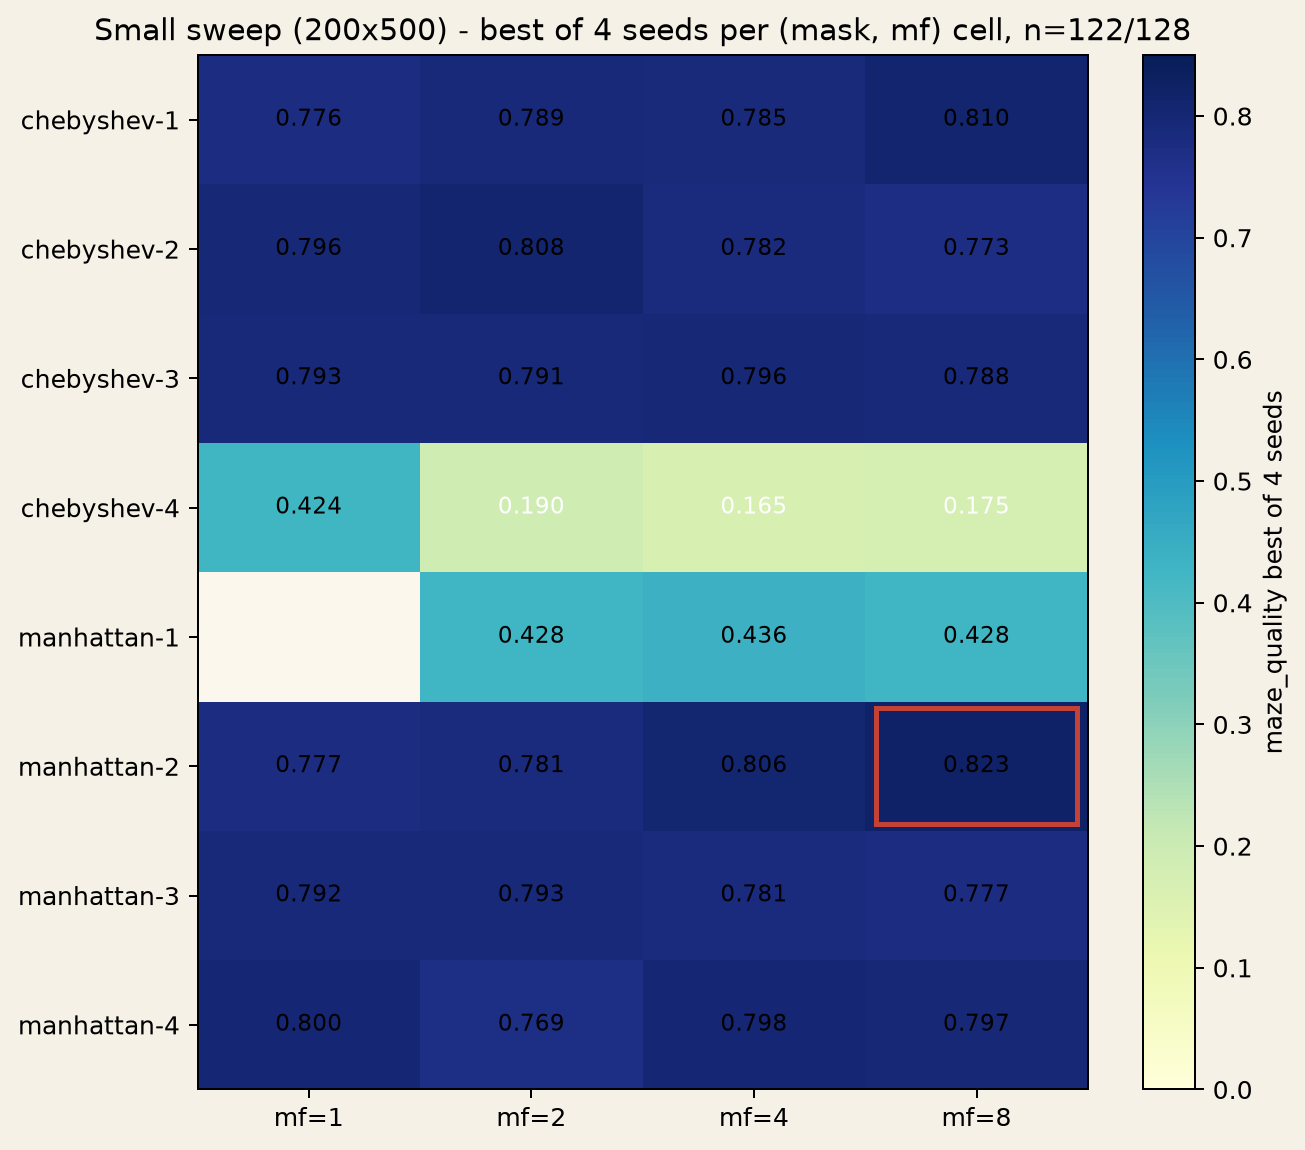
\includegraphics[width=0.96\linewidth]{../figures/v2/fig_smallsweep_heatmap.png}
\caption{\textbf{小范围 sweep ($200 \times 500$) 122 个 OK run 的 (mask, maxFam) 汇总。}
每格数值 = 该 (mask, maxFam) 上 4 个随机种子中的最高 $maze\_quality$。
红框 = 全场峰值 (manhattan-2 / maxFam=8, $0.8233$)。
8 个 mask 中 6 个健康 ($0.74$--$0.78$), 2 个异常: chebyshev-4 (0.157) 与 manhattan-1 (0.421),
机制完全不同 (见 §6.2)。
n=122/128, 缺失的 6 个为 TIMEOUT。}
\label{fig:smallsweep-heatmap}
\end{figure}

按 mask 分组均值见表~\ref{tab:mask-mean-v13}。8 个 mask 中 6 个健康 (chebyshev-1/2/3, manhattan-2/3/4 均值 $\ge 0.74$), 2 个异常 (chebyshev-4 = 0.157, manhattan-1 = 0.421)。

\begin{table}[H]
\centering\small
\caption{小范围 sweep 按 mask 模板的均值 / 最小 / 最大 (n=122)}
\label{tab:mask-mean-v13}
\begin{tabular}{lccccc}
\toprule
\textbf{mask} & \textbf{n} & \textbf{mean} & \textbf{min} & \textbf{max} & \textbf{状态} \\
\midrule
chebyshev-1    & 16 & 0.7726 & 0.7279 & 0.8095 & healthy \\
chebyshev-2    & 16 & 0.7438 & 0.5909 & 0.8080 & healthy (高方差) \\
chebyshev-3    & 16 & 0.7764 & 0.7446 & 0.7955 & healthy \\
chebyshev-4    & 16 & 0.1573 & 0.1038 & 0.4244 & 低均值 (预算受限) \\
manhattan-1    & 10 & 0.4205 & 0.3998 & 0.4360 & 低均值 (表征受限) \\
manhattan-2    & 16 & 0.7777 & 0.7429 & \textbf{0.8233} & healthy (最优) \\
manhattan-3    & 16 & 0.7714 & 0.7014 & 0.7932 & healthy \\
manhattan-4    & 16 & 0.7517 & 0.4452 & 0.7999 & healthy (高方差) \\
\bottomrule
\end{tabular}
\end{table}

按 maxFam 分组: mf=1 均值 0.6984 (n=28), mf=2 均值 0.6688 (n=30), mf=4 均值 0.6382 (n=32), mf=8 均值 0.6306 (n=32)。均值随 maxFam 单调下降, 但峰值从 mf=1 的 0.7999 升至 mf=8 的 0.8233 --- ``均值降, 峰值升'' 现象。

\subsection{小范围 vs 大范围对比}

小范围 sweep 122 个 OK run 提供完整的 (mask, maxFam) 消融数据 (§5.3); 大范围 sweep 的 5/5 run 提供 ``同配置, 大网格'' 的 scale-up 证据 (§5.2)。两者对比要点:
\begin{itemize}[leftmargin=*, itemsep=0pt, topsep=0pt]
  \item \textbf{配置覆盖}. 大范围只测了 manhattan-2 / maxFam=8 一种配置, 小范围测了 $8 \times 4 = 32$ 种 (mask, maxFam) 组合。
  \item \textbf{网格面积}. 大范围 $500 \times 2000 = 10^6$ 像素, 小范围 $40 \times 60 = 2400$ 像素, 大范围约高 417 倍。
  \item \textbf{峰值差}. 大范围 5-run 最高 0.8195, 小范围单点最高 0.8233, 差 0.0037。
  \item \textbf{解释}. manhattan-2 / maxFam=8 在 $40 \times 60$ 网格上已接近该配置的理论上界 (见 §6.3); 大范围 sweep 用于验证 ``峰值不显著下降'' 而非 ``寻找新高分''。
\end{itemize}

\subsection{数据来源声明}

所有数值以 append-only ndjson 训练日志为唯一来源, 不以 ckpt 文件为数值依据:
\begin{itemize}[leftmargin=*, itemsep=0pt, topsep=0pt]
  \item 小范围 sweep ndjson: \texttt{sweep\_2026\_07\_04/results.ndjson} (122 OK + 6 TIMEOUT)。
  \item 大范围 sweep ndjson: \texttt{sweep\_2026\_07\_08\_big/results.ndjson} (5 OK)。
  \item 15-pattern 对照基准: 图案 \texttt{paper/data/\_grids.json} (15 张 31$\times$31 网格, 0/1 flat), 分数 \texttt{paper/data/sweep\_summary.json::15pattern.per\_pattern}, 复核脚本 \texttt{paper/data/\_eval\_15patterns.mjs} (15/15 数值精确匹配, 详见附录 B)。
\end{itemize}
